\question \textbf{Affine gap with single DP table}
  
You need to check extra cells in addition to the adjacent cells of H when finding an optimal alignment with affine gap penalties.

\medskip 

\textbf{Scoring scheme: }\\
\null \quad $R_{ab}$ = 1 for a = b \\ 
\null \quad $R_{ab}$ = 0 for a $\neq$ b \\ 
\null \quad $g_{open} = 1$, $g_{extend} = 0.1 $ 

\begin{figure}[h]
  \centering
      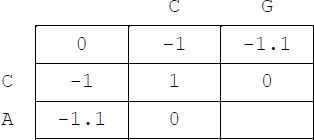
\includegraphics[width=0.3 \textwidth]{fig03/affine_gap_single_table.png}
\end{figure}

Assume we want to update $H_{2,2}$ and answer the following questions.

\newpage

\begin{parts}

%% (a)
  \part
  Calculate $H_{1,1} + R_{q_2, d_2}$.
    
  \begin{solution}[0.35 in]
  $1 + 0 = 1$
  \end{solution}

%% (b)
  \part
  Calculate $max_{1 \leq l \leq 2}(H_{2,2-l} - g_{l})$.

  \begin{solution}[0.35 in]
  $max⁡(H_{2,1} - g_{l=1}, H_{2,0} - g_{l=2}) = max(0 - 1, -1.1 - 1.1) = -1$
  \end{solution}
  
%% (c)
  \part
  Calculate $max_{1 \leq l \leq 2}(H_{2-l,2} - g_{l})$.

  \begin{solution}[0.35 in]
  $max⁡(H_{1,2} - g_{l=1}, H_{0,2} - g_{l=2}) = max(0 - 1, -1.1 - 1.1) = -1$
  \end{solution}
  
 %% (d)
  \part
  What is the score of $H_{2,2}$.
  
  \begin{solution}[0.35 in]
  $max(1, – 1,  -1) = 1$
  \end{solution}
     
  \vspace{0.1 in}

\end{parts}